\section{Evaluation Results}
\label{sec:evaluationresults}

In this section we discuss our experiments and results. We chose accuracy as our evaluation metric when comparing different models. For brevity, we are reporting the accuracy numbers to two decimal places. 

For Section~\ref{subsec:linearclassifiersonrawimagepixels}, Section~\ref{subsec:neuralnetworksonrawimagepixels} and Section~\ref{subsec:imagefeatures} we re-purposed code from assignments 1 and 2 in Stanford University's Spring 2017 course, CS231N: Convolutional Neural Networks for Visual Recognition~\cite{cs231n}. For Section~\ref{subsec:convolutionalnetworks} and Section~\ref{subsec:transferlearning}, we use TensorFlow~\cite{abadi2016tensorflow} for training our convolutional network models.

\begin{table*}[h!]
\begin{center}
\begin{tabular}{|l|c|c|}
\hline
Modeling Approach & Best Validation Accuracy & Test Set Accuracy \\
\hline\hline
Linear SVM on raw image pixels & 0.18 & 0.16 \\
Five layer fully connected neural net on raw image pixels & 0.19 & 0.18 \\
Linear SVM on image features & 0.21 & 0.22 \\
Two layer neural net on image features & 0.26 & 0.27 \\
Training a Convolutional Network from scratch  & 0.40 & 0.40 \\
Transfer Learning (by fine tuning a VGG model) & 0.46 & 0.45 \\
\hline
\end{tabular}
\end{center}
\caption{Summary of results across different modeling approaches.}
\label{table:accuracyresults}
\end{table*}

\subsection{Linear classifiers on raw image pixels}
\label{subsec:linearclassifiersonrawimagepixels}

%\begin{figure} 
%\centering
%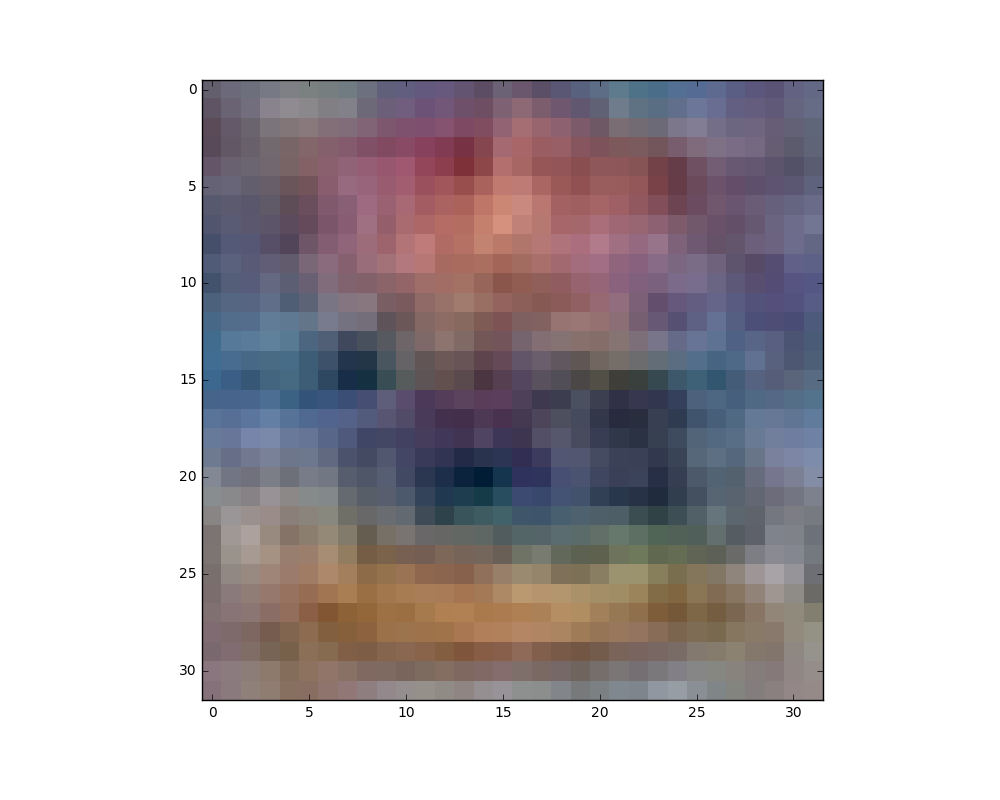
\epsfig{file=Figs4Paper/_final/svm_learnedweights_burger.eps, height=1.25in, width=1.6in} 
%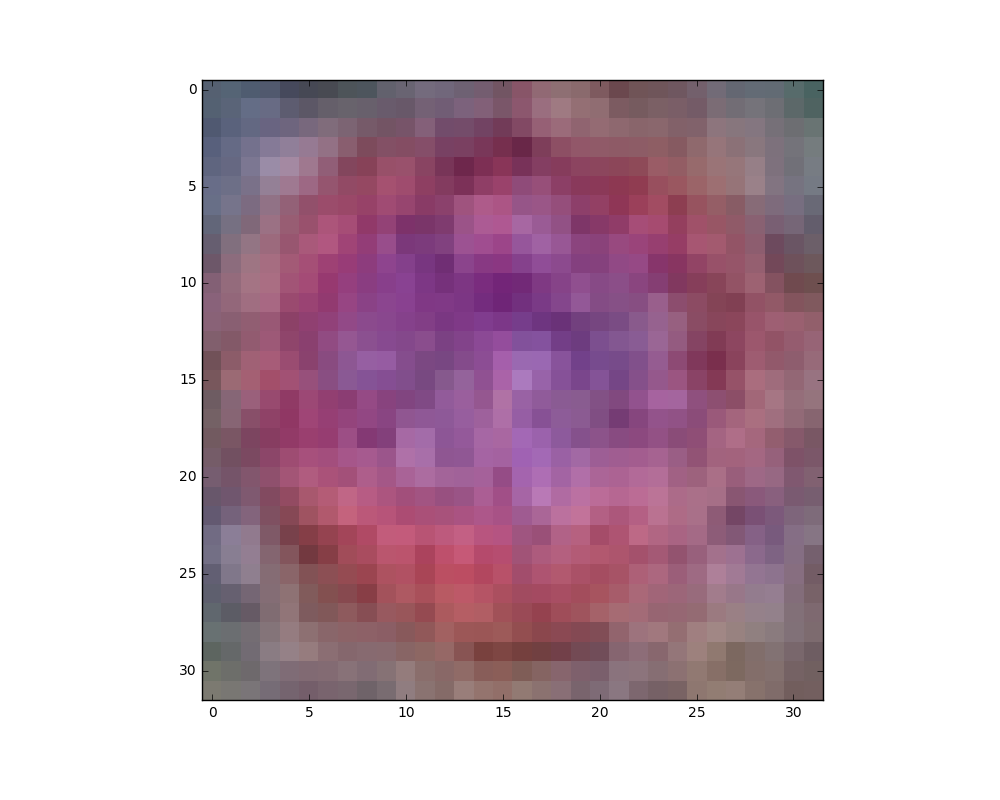
\epsfig{file=Figs4Paper/_final/svm_learnedweights_pizza.eps, height=1.25in, width=1.6in}
%\caption{Visualizing the weights learned by the SVM model for the burger and pizza classes}
%\label{fig:learnedweightsburgerpizza}
%\end{figure}

\begin{figure}[ht!]
    \centering
    \begin{subfigure}{.4\linewidth}
        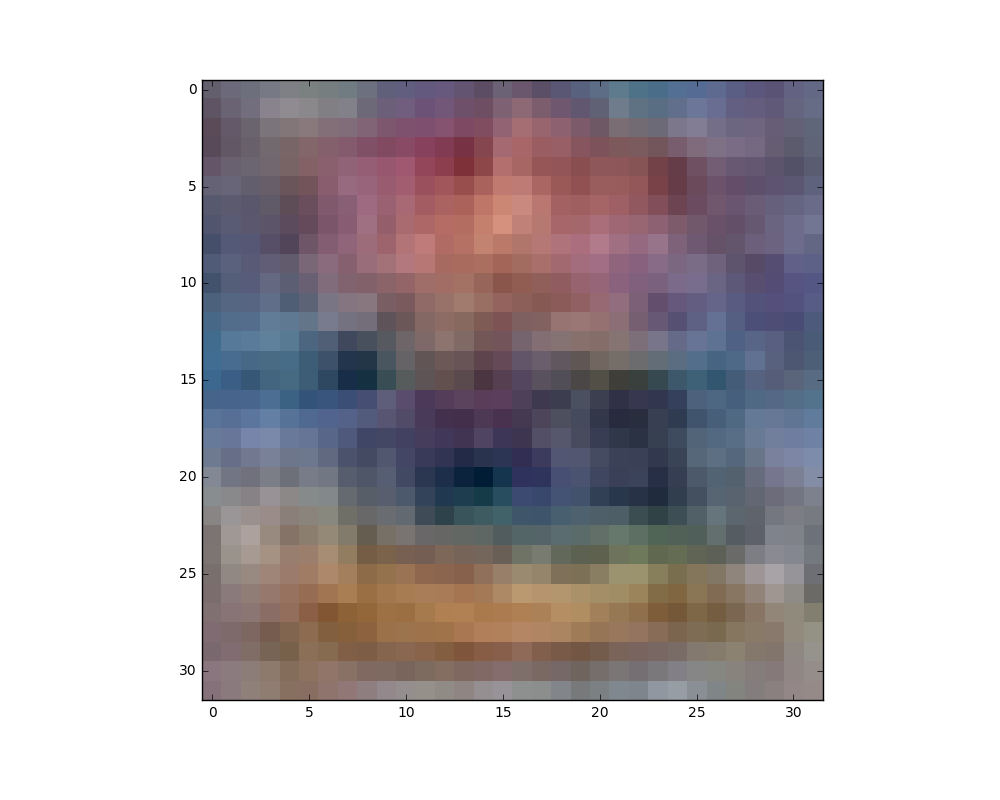
\includegraphics[height=1.25in, width=1.6in]{Figs4Paper/_final/svm_learnedweights_burger.eps}
        \caption{burger}
    \end{subfigure}
    \hskip2em
    \begin{subfigure}{.4\linewidth}
        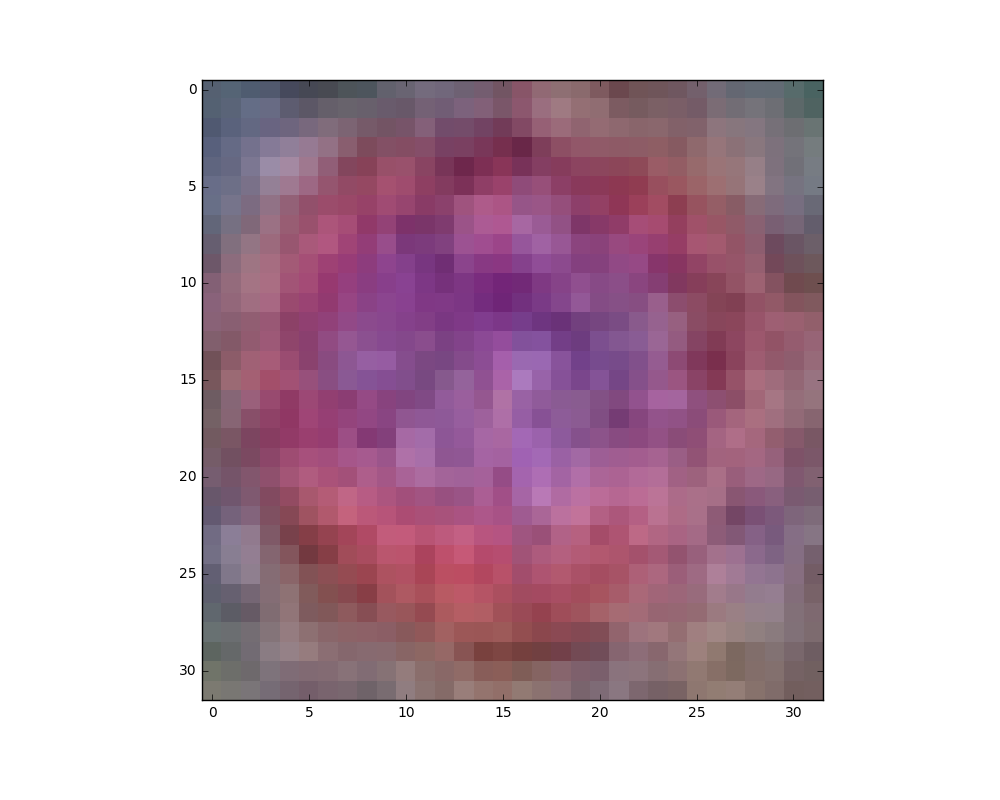
\includegraphics[height=1.25in, width=1.6in]{Figs4Paper/_final/svm_learnedweights_pizza.eps}
        \caption{pizza}
    \end{subfigure}
    \caption{Visualizing the weights learned by the SVM model}
		\label{fig:learnedweightsburgerpizza}
\end{figure}


To set our baseline, we first use a linear classifier using raw image pixels as features. For this we tried out both a SVM classifier and a Softmax classifier. The best validation accuracy of 0.18 was achieved using the SVM classifier with a learning rate 1e-07 and regularization strength 2.5e+04. The corresponding test set accuracy was 0.16.

One interpretation of a linear classifier is that of a \textit{template match}, where each row of the learned weights matrix corresponds to a template for the corresponding class. Figure~\ref{fig:learnedweightsburgerpizza} shows the learned weights for the burger and pizza classes in our dataset. We note that both the templates match our intuition; the burger contains a lot of brown pixels, the pizza has a round shape and contains a lot of red pixels at the center.   

\subsection{Neural networks on raw image pixels}
\label{subsec:neuralnetworksonrawimagepixels}

\begin{figure}[h!]
\centering
  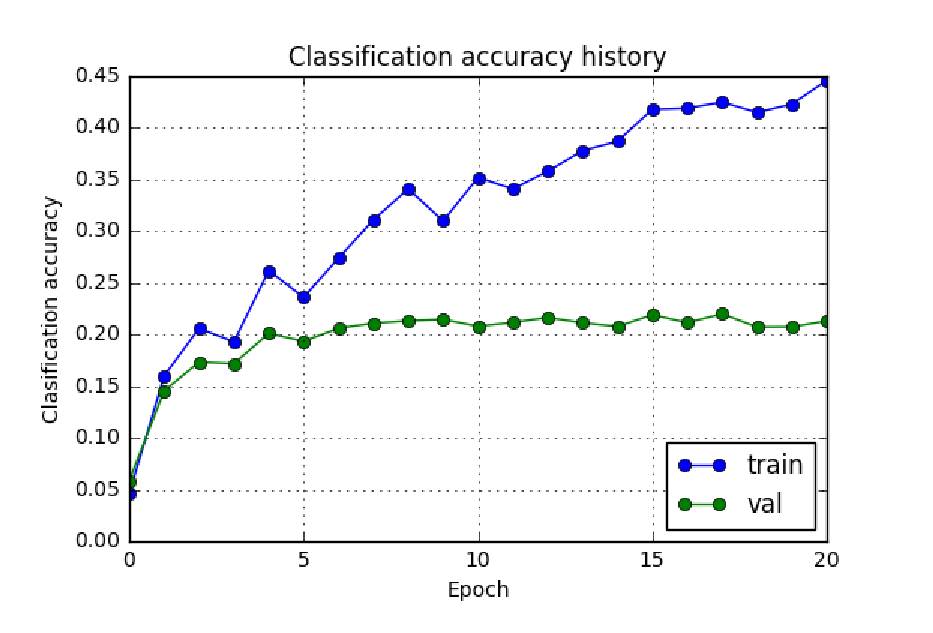
\epsfig{file=Figs4Paper/_final/fcfivelayer_rawpixels_classificationaccuracy.eps, height=1.5in, width=2.5in}
  \caption{Classification accuracy history of a fully connected five layer neural network using raw image pixels}
  \label{fig:fcfivelayerrawpixelsclassificationaccuracy}
\end{figure}

The next set of models we tried out were fully connected neural networks, again using raw image pixels as features.  Our network architecture was a six layer fully-connected network. Each of the five hidden layers had 100 neurons each. We used ReLU nonlinearity, and a softmax loss function. Below we note some interesting observations from training these models.

\begin{itemize}[noitemsep]
\item Batch normalization was~\cite{ioffe2015batch} \textbf{very useful} in training our model. Without batch normalization our model was performing quite poorly.
\item The best validation accuracy of 0.19 was achieved using the \textbf{Adam}~\cite{kingma2014adam} update rule with a learning rate of 1e-03. The test set accuracy was 0.18   
\end{itemize}

Figure~\ref{fig:fcfivelayerrawpixelsclassificationaccuracy} shows the classification loss history for the training and validation sets over 20 epochs while training this network.

\begin{figure*}[h!]
\centering
	\fbox{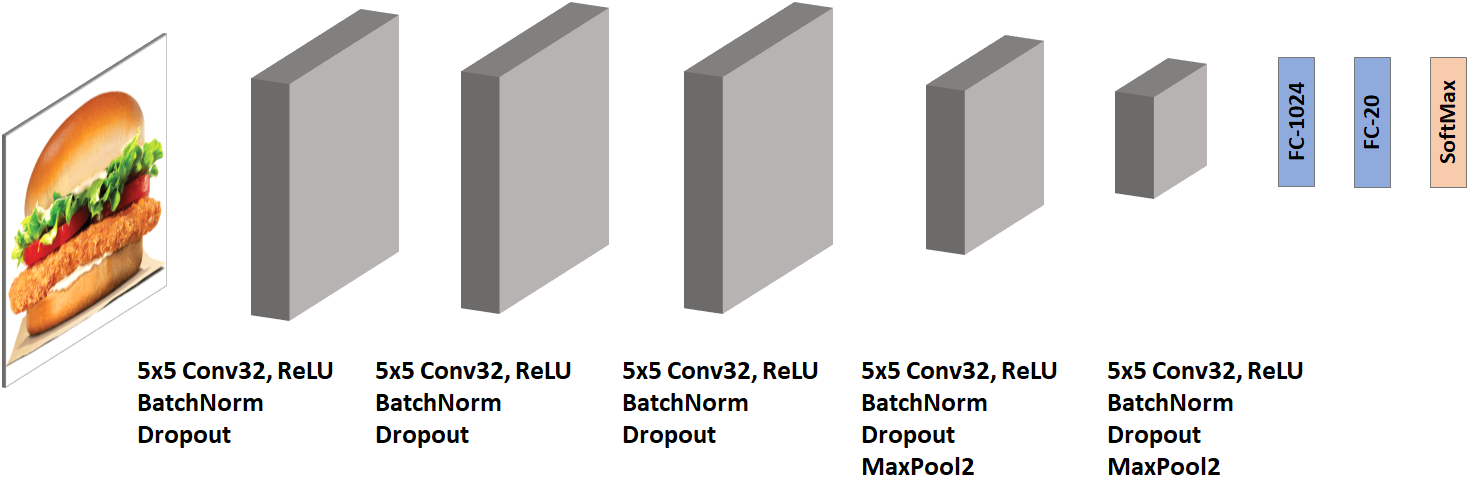
\includegraphics[width=12cm]{Figs4Paper/_final/convnet_architecture.eps}}
  \caption{Convolutional network architecture}
  \label{fig:convnetarchitecture}
\end{figure*}

\subsection{Image features}
\label{subsec:imagefeatures}


\begin{figure}[h!]
\centering
  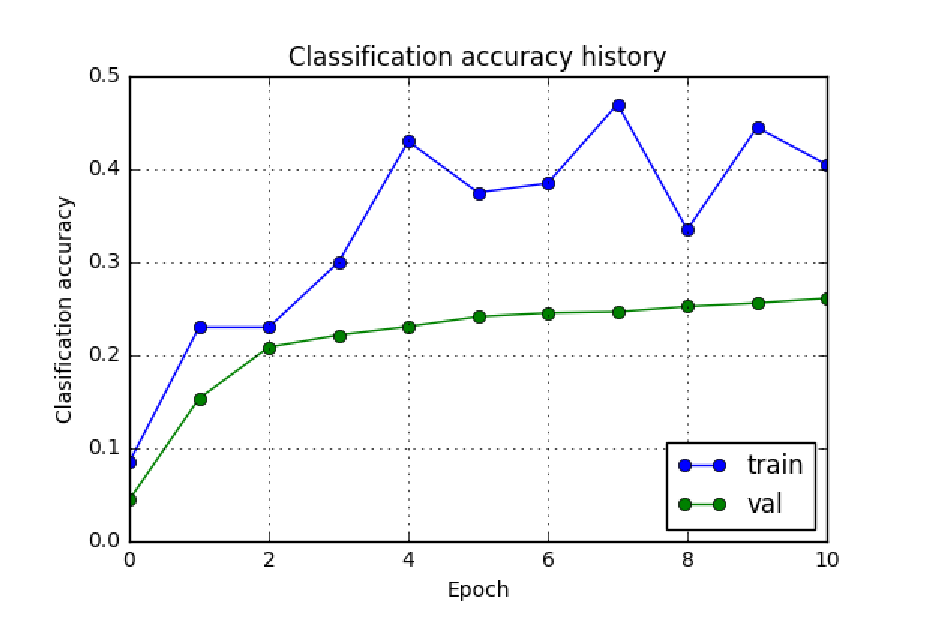
\epsfig{file=Figs4Paper/_final/imagefeatures_fctwolayer_classificationaccuracy.eps, height=1.5in, width=2.5in}
  \caption{Classification accuracy history of a fully connected two layer neural network using image features}
  \label{fig:imagefeaturesfctwolayerclassificationaccuracy}
\end{figure}

We did a set of experiments using features extracted from the images. For featurizing each image, we compute a Histogram of Oriented Gradients (HOG) as well as a color histogram using the hue channel in HSV color space. We form our final feature vector for each image by concatenating the HOG and color histogram feature vectors. This gives us a total of 155 features for each image. Below we summarize the results using image features with a SVM and a Two Layer Fully Connected Neural Network classifier.

\begin{itemize}[noitemsep]
\item Using the images features with a linear SVM classifier we were able to get a validation accuracy of 0.21, using SGD with a learning rate of 1e-03 and regularization strength of 1e+00
\item Using the images features with a Two Layer Fully Connected Neural Network gave much better performance. We got the best validation accuracy of 0.26 while using SGD as our update rule with a learning rate of 0.9, learning rate decay of 0.8 and regularization strength 0. The corresponding test set accuracy was 0.27   
\end{itemize}

Figure~\ref{fig:imagefeaturesfctwolayerclassificationaccuracy} shows the classification loss history for the training and validation sets over 10 epochs while training the Two Layer Fully Connected Neural Network classifier with image features.

\subsection{Convolutional Networks}
\label{subsec:convolutionalnetworks}

Using Convolutional Networks we were able to get the validation and test set accuracy of 0.40 each. Figure~\ref{fig:convnetarchitecture} shows the architecture we used. Below we note some of the things we tried out.

\begin{itemize}[noitemsep]
\item Batch normalization~\cite{ioffe2015batch} was quite useful in training our model.
\item For the weights in our network, using Xavier initialization~\cite{glorot2010understanding} helped.
\item Dropout~\cite{hinton2012improving, srivastava2014dropout} (with keep probability 0.75) helped improve the validation accuracy from 0.38 to 0.40. 
\item We kept the number of filters fixed at 32. 
\item We tried different sized filters (3x3, 5x5 and 7x7) but they did not help much. So we fixed the filter size at 5x5.
\item For the first three conv layers we preserve the height and width dimensions. For the fourth and fifth conv layers, we used max pooling with stride 2 (across both height and width).
\item After the five conv layers, we added two fully connected layers with 1024 and 20 neurons respectively. 
\item For the last layer we use softmax with cross entropy loss. 
\item The best validation accuracy of 0.40 was achieved using the \textbf{Adam}~\cite{kingma2014adam} update rule with a learning rate of 1e-04. The test set accuracy was 0.40. 
\end{itemize}

\begin{figure}[h!]
\centering
  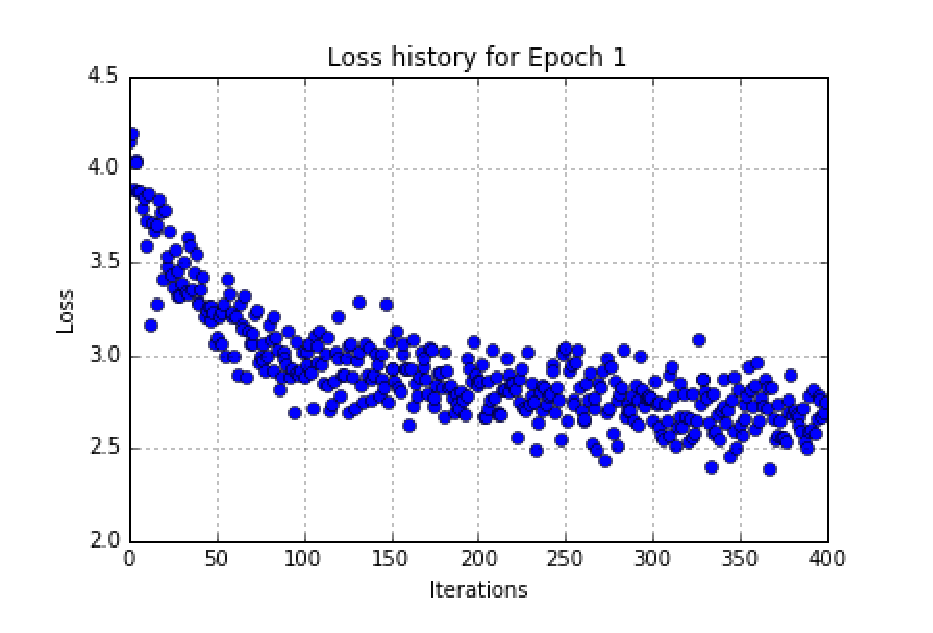
\epsfig{file=Figs4Paper/_final/convnet_losshist_epoch1.eps, height=1.5in, width=2.5in}
  \caption{Reduction in loss over several mini-batches in the first epoch of the convolutional network}
  \label{fig:lossepoch1}
\end{figure}

Figure~\ref{fig:lossepoch1} shows the reduction in the loss over multiple iterations in the first epoch. We see the loss reduces very sharply in the beginning, and then flattens out gradually.  

\begin{figure}[h!]
\centering
  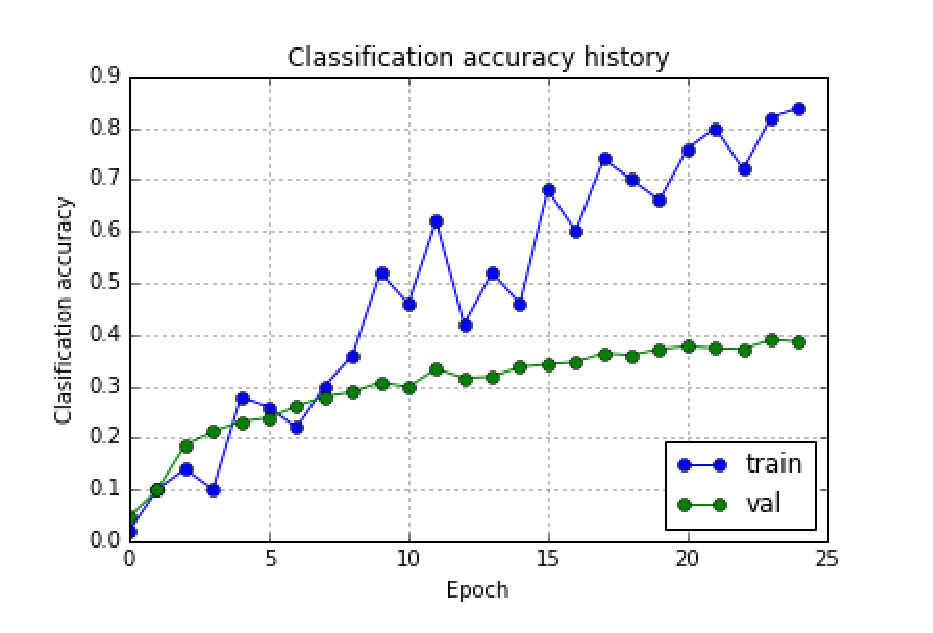
\epsfig{file=Figs4Paper/_final/convnet_classificationaccuracy.eps, height=1.5in, width=2.5in}
  \caption{Classification accuracy history of the convolutional network over 25 epochs}
  \label{fig:convnetclassificationaccuracy}
\end{figure}

Figure~\ref{fig:convnetclassificationaccuracy} shows the classification loss history for the training and validation sets over 25 epochs of the conv net.

\subsection{Transfer Learning}
\label{subsec:transferlearning}

\begin{figure}[h!]
\centering
  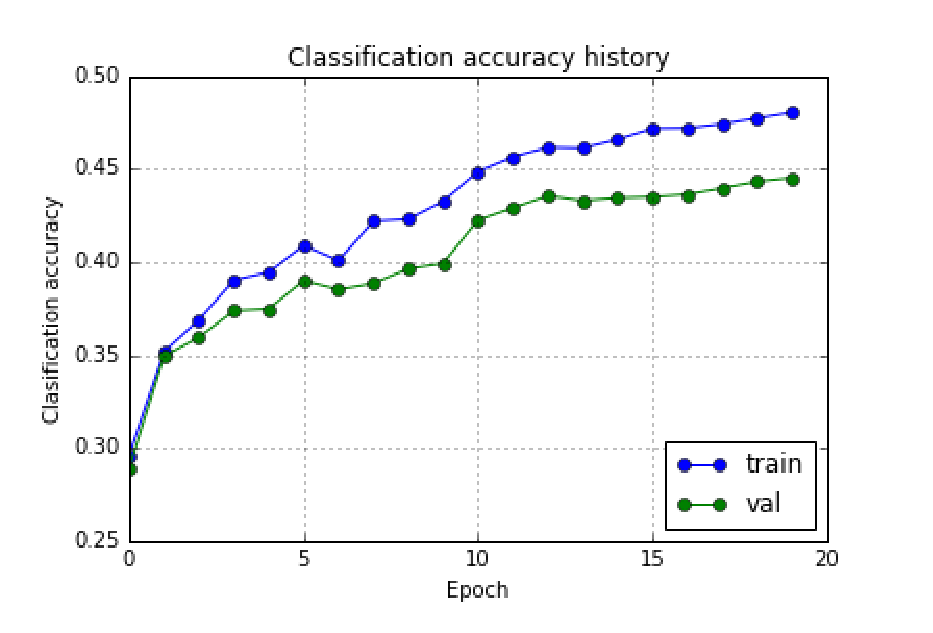
\epsfig{file=Figs4Paper/_final/transferlearning.eps, height=1.5in, width=2.5in}
  \caption{Classification accuracy history after fine-tuning a VGG model}
  \label{fig:transferlearning}
\end{figure}

To improve the accuracy of our model further, we did a set of experiments around transfer learning. Interestingly this gave us the best results on our dataset.  Some salient observations from this approach are as follows:

\begin{itemize}[noitemsep]
\item We are using the VGG-16~\cite{simonyan2014very} model pretrained on ImageNet
\item We remove the last fully connected layer (fc8) and replace it with our own, with output size 20
\item We first train the last layer for 10 epochs. This allows us to get meaningful weights for the fc8 layer first.  Subsequently, we train the entire model on our dataset for 10 more epochs.
\end{itemize}

For this approach, we referenced the TensorFlow finetune sample on GitHubGist~\cite{finetunegithubgist}. Following the example in the gist, we did similar pre-processing on our dataset to make it work for the VGG-16 model. The pre-processing steps are listed below:

\begin{itemize}[noitemsep]
\item Resize the image so its smaller side is 256 pixels long. Recall that our existing dataset has dimensions (32, 32, 3).
\item Take a random 224x224 crop of the scaled image (for the train, validation and test sets)
\item Horizontally flip the image with probability 1/2 (for the train set only)
\item Substract the per color mean VGG\_MEAN [123.68, 116.78, 103.94) (for the train, validation and test sets)
\end{itemize}


Figure~\ref{fig:transferlearning} shows the classification loss history for the training and validation sets over all the 20 epochs. Table~\ref{table:accuracyresults} shows a summary of results across different modeling approaches.




